\documentclass{standalone}
\usepackage{pgfplots}
\begin{document}
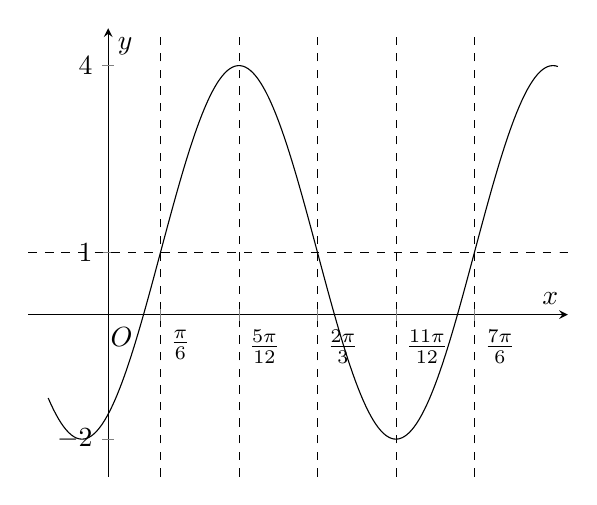
\begin{tikzpicture}
\begin{axis}
[
ymin=-2.6,ymax=4.6,
xmin=-0.8,xmax=4.6,
xtick=\empty,
ytick=\empty,
extra x ticks={0.5236, 1.309, 2.0944, 2.87979, 3.66519},
extra x tick labels={$\frac{\pi}{6}$, $\frac{5\pi}{12}$, $\frac{2\pi}{3}$, $\frac{11\pi}{12}$, $\frac{7\pi}{6}$},
extra y ticks={-2, 1, 4},
extra y tick labels={$-2$, $1$, $4$},
every extra x tick/.style={
    xticklabel style={anchor=north west},
    grid=major,
    major grid style={very thin,dashed,black}
},
axis lines = center,
xlabel=$x$,ylabel=$y$,
samples=200,
]
\addplot [black, domain=-0.6:4.5] {3*sin(deg(2*x - pi/3)) + 1};
\addplot [black, dashed, domain=-0.8:4.6] {1};
\node at (axis cs:0.135, -0.36) {$O$} ;
\end{axis}
\end{tikzpicture}
\end{document}
